%%% Intro.tex --- 
%% 
%% Filename: Intro.tex
%% Description: 
%% Author: Ola Leifler
%% Maintainer: 
%% Created: Thu Oct 14 12:54:47 2010 (CEST)
%% Version: $Id$
%% Version: 
%% Last-Updated: Thu May 19 14:12:31 2016 (+0200)
%%           By: Ola Leifler
%%     Update #: 5
%% URL: 
%% Keywords: 
%% Compatibility: 
%% 
%%%%%%%%%%%%%%%%%%%%%%%%%%%%%%%%%%%%%%%%%%%%%%%%%%%%%%%%%%%%%%%%%%%%%%
%% 
%%% Commentary: 
%% 
%% 
%% 
%%%%%%%%%%%%%%%%%%%%%%%%%%%%%%%%%%%%%%%%%%%%%%%%%%%%%%%%%%%%%%%%%%%%%%
%% 
%%% Change log:
%% 
%% 
%% RCS $Log$
%%%%%%%%%%%%%%%%%%%%%%%%%%%%%%%%%%%%%%%%%%%%%%%%%%%%%%%%%%%%%%%%%%%%%%
%% 
%%% Code:


\chapter{Integration of Optimization toolchain into the Model-Based Development Process}
\label{cha:optimization}


\section{Introduction}
\label{sec:optimizationintroduction}

Equation-based, object-oriented modelling languages such as Modelica  have become increasingly used for
industrial applications. These languages enable users to conveniently model large-scale physical systems described by 
differential, algebraic, and discrete equations, primarily with the goal of performing virtual experiments (simulation) 
on these systems, but recently also optimization.

During the last decade, nonlinear model predictive control (NMPC) and nonlinear optimal control problems (NOCP)
based on differential-algebraic equations (DAE) have had a significant impact in the industrial community, particularly in
the control engineering area \cite{biegler, tamimi}. State-of-the-art methods are using numerical
algorithms for dynamic optimization based on direct multiple shooting \cite{bock} or collocation algorithms
\cite{biegler}.

Due to the influence of such equation-based, object-oriented modeling languages in the industrial community, there have
been several attempts to integrate tools for such languages with numerical algorithms for optimization. For example,
Dymola (DassaultSystemes, 2010) supports parameter and design optimization of models written in Modelica whereas
JModelica.org \cite{akesson} and OpenModelica \cite{bernhard} have native support for optimal
control.

This chapter presents results of an effort where model-based dynamic optimization has been done by integrating
OpenModelica and CasADi \cite{casadi}. The problem formulation and modeling is done in Modelica 
(Modelica Association, 2010) including the optimization \cite{optimica} language extension. The integration is based
on standardized XML format presented in \cite{xml} for exchange of differential-algebraic equations (DAE)  models. 
OpenModelica supports export of models written in Modelica and the optimization language extension using this XML 
format, while CasADi supports import of models represented in this format. This allows users to define optimal control problems (OCP) using
Modelica and optimization language specification, and solve the underlying model formulation using a
range of optimization methods, including direct collocation and direct multiple shooting. The proposed
solution has been tested on several industrially relevant optimal control problems, including a dieselelectric
power train.

\section{Nonlinear Optimal Control Problems (NOCP)}
\label{sec:optimizationnocp}

Model-based optimization results in nonlinear optimal control problems of the form \cite{friesz}:

\begin{equation} \label{eq:1}
    \text{min}\; M \Big(x(t_f )\Big)+\int_{(t_0)}^{(t_f)}\; L(x(t),u(t),t) dt 
\end{equation}

subject to

\begin{equation} \label{eq:2}
	 r_0\Big(x(t_0),\dot{x}(t_0)\Big) = 0 
\end{equation}
\begin{equation}\label{eq:3}
	 0 = fx(t),\dot{x}(t),u(t),t\Big)
\end{equation}
\begin{equation}\label{eq:4}
	0 \leq g\Big(x(t),x(t),u(t),t\Big)
\end{equation}
\begin{equation}\label{eq:5}
	r_f\Big(x(t_f),\dot{x}(t_f)\Big)
\end{equation}

where $ t \in [t_0,t_f ] $ is the time, $ x(t) \in {\mathbb{R}}^ {n_x} $ are state variables and  $ u(t) \in {\mathbb{R}}^ {n_u}$ are control variables. Initial and terminal equations are \ref{eq:2} and \ref{eq:5}, respectively. Equation \ref{eq:4} represents path constrains and. Equation \ref{eq:3} is the nonlinear dynamic model description given as a differential-algebraic equation (DAE). The objective function \ref{eq:1} is composed of an end cost (Mayer term) and an integral cost (Lagrange term).

\section{Numerical handling}
\label{sec:numericalhandling}

For the numerical solution, the time horizon,$ [t_0,t_f] $, will be divided into a finite number of intervals $[t_0,t_1 ],…,[t_{n-1},t_n ]$, e.g. equidistant partitioning:

\begin{equation*}
	t_i\quad:=\quad t_0+h.i,i=0,...,n,h:= \frac{t_f-t_0}{n} 
\end{equation*}

A good approximation for the Lagrange term in a subinterval $[t_i,t_{i+1}]$ is given by Gaussian quadrature. For that, intermediate points $x(t_i+s_k.h)$ with $s_k\in [0,1]$ and respective weights $ w_k $ are needed. This requirement naturally induces for the discretization of \ref{eq:3} so-called collocation methods. There are special classes related to implicit Runge-Kutta methods \cite{deuflhard}. In order to achieve continuous solutions with minimal expenditure it is requested that the endpoints are included in the collocation scheme \cite{bernhard}). Therefore, the Radau IIA or Lobatto IIIA formulas can be used \cite{hermann}. The main differences between the two methods are that the Radau IIA has a higher stability. On the other hand, Lobatto IIIA includes the start point and it is possible to accomplish differentiable solutions. This is important if initial equations also have constraints on the derivatives.

\section{Total Collocations}
\label{sec:totalcollocations}

Applying implicit Runge-Kutta methods for local approximation of equation \ref{eq:3} leads to a system of nonlinear equations for each subinterval. The exact solution of each nonlinear equation system can be spared by adding these to the over-all nonlinear problem \cite{biegler} which leads to the total collocation method. The finite dimensional optimization problem is finally described by the nonlinear programming problem (NLP):

\begin{equation}\label{eq:6}
   \text{min} \; M\quad(x_{m,n}) + h\quad.\quad \sum_{j=0}^{m} w_j\quad .\quad\sum_{i=0}^{n} L(x_{j,i},u_{j,i}, t_{j,i} )
\end{equation}

subject to

\begin{equation}\label{eq:7}
	\begin{aligned}
		r_0(x_{0,0}) = 0 \\
		res(x_{k,i}, u_{k,i}, t_{k,i} ) = 0 \\
		g(x_{k,i}, u_{k,i}, t_{k,i} ) \geq 0 \\
		r_f(x_{m,n} = 0
	\end{aligned}
\end{equation}

where $ t_{k,i} = t_i+s_k.h $ are time points for the collocation residuals, $ x_{k,i} \approx x(t_{k,i}) $ are the approximation which are implicit given by the fulfilment of the conditions and $ u_{k,i}= u(t_{k,i}) $  for $ k=1,..m $ and $ i=0,..m.$ For the case $t_f$ is free then the optimization problem will be harder and the initial guess will be more important. $ res(x_{k,i},u_{k,i},t_{k,i} )$ are collocation residuals. More detailed descriptions are in \cite{bernhard}. Note, equation \ref{eq:3} is usually given in implicit form. For efficiency reason it is quite important to use the symbolic pre-processing already available within the tool chain to transform equation \ref{eq:3} to semi-explicit DAE of index 1. This procedure will reduce the solution space dramatically and might be a prerequisite for finding a solution to the non-linear problem \ref{eq:7}.

\section{CasADi}
\label{sec:optcasadi}

CasADi \cite{casadi} is an open-source framework for C++ and Python for numerical optimization in general and optimal control in particular. The main idea of the tool is to provide users with the ability to easily and efficiently implement optimal control algorithms with a wide range of methods, including multiple shooting and collocation, rather than providing users with a “black-box” OCP solver.
The tool supports symbolic import of OCPs via an extended version of the functional mockup interface (FMI) format as explained in \cite{optandersson}. This OCP can then be transcribed into a nonlinear programming problem (NLP) using the approach outlined in Section 2.2, and solved with one of CasADi’s interfaced NLP solvers.

\section{Modelica and the Optimization Language Extension}
\label{sec:optimizationoptimica}

Modelica is a mature and powerful language regarding modelling of complex hybrid dynamical systems. However, it
lacks important features for describing or modelling optimization problems. This is not a surprise since Modelica
was not originally designed to help with dynamic optimization problems.

The optimization language extension \cite{optimica} complements Modelica by providing features which enable
formulation of dynamic optimization problems based on Modelica models. The optimization extension to Modelica
consists of the following elements:

\begin{itemize}
	
\item \textit{objective} and \textit{objectiveIntegerand}, which maps the Mayer and the Lagrange term in 
             the objective function \ref{eq:1} respectively.
\item \textit{startTime}, which defines the start of the optimization interval.
\item \textit{finalTime}, which defines the end of the optimization interval.
\item A new section: \textit{constraint}, which defines inequality constraints.
\end{itemize}

The requirement and motivation for introducing these specific features is covered in more detail in \cite{optimica}.

\section{OpenModelica Compiler and XML Export}
\label{sec:optimizationopenmodelica}

The OpenModelica compiler front-end has been extended to support the optimization language extension described in
section 4. This enable users to formulate and use modelbased NOCP that can be solved by CasADi, In addition, the
OpenModelica compiler has recently been extended with XML export of models \cite{alachew} based on the XML
format defined in \cite{xml}. This schema is an extended version of the XML schema
defined by the Functional Mock-up Interface (FMI) (Modelisar, 2010), and is the most recent in a series of
Modelica-related XML schemas starting with ModelicaXML \cite{pop}.The XML export also includes the
optimization language extension, and OpenModelica is integrated with CasADi for model-based dynamic optimization reported in this thesis.

\section{Complete Tool Chain}
\label{sec:optimizationtoolchain}

Before exporting a Modelica and optimization language model to XML, the model should be symbolically
instantiated by the compiler in order to get a single flat system of equations. The model variables should also be
scalarized. The compiler frontend performs this, including syntax checking, semantics and type checking, simplification
and constant evaluation etc. are applied. Then the complete flattened model is exported to XML code. The exported
XML document can then be imported to CasADi for modelbased dynamic optimization. The complete tool chain is
visualized in Figure \ref{fig:optimizationtoolchain}.

\begin{figure}
	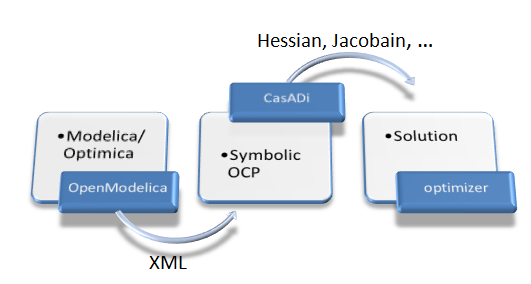
\includegraphics[width=\linewidth]{opt_tool_chain.png}
	\caption{Optimization tool chain for OpenModelica and CasADi.}
	\label{fig:optimizationtoolchain}
\end{figure}

The XML will be imported and symbolically pre-processed in CasADi. In particular, the fully-implicit DAE from
Modelica is reformulated in a semi-explicit form. With the NOCP now available in CasADi’s native data structures, the
NOCP can be reformulated to a NLP as outlined in Section \ref{sec:totalcollocations}.

At the time of writing, the efficient symbolic pre-processing model evaluation from OpenModelica is not yet completely
implemented to import into CasADi. So the symbolic preprocessing in CasADi can be used. The symbolic work in CasADi makes it easy to create the goal function \ref{eq:6} and constraints \ref{eq:7}.

The NLP is solved by one of the NLP solvers interfaced to CasADi, e.g. IPOPT \cite{wachter}. First and second order derivative information will be generated by CasADi using automatic differentiation and passed to the solver.

\section{Testing the Implementation}
\label{sec:optimizationtesting}

In this chapter, we describe the solution of an industrial-relevant optimal control problem of the diesel electric powertrain. The
formulation of the underlying optimization problem and the corresponding optimization results are presented in the
following subsections.

\subsection{Fuel optimal control of a diesel electric powertrain}
\label{sec:optimizationdiesel}

The diesel-electric powertrain model presented in \cite{sivertsson,bernhard} is a nonlinear
mean value engine model (MVEM) containing four states and three control inputs while the generator model is
simplified by considering constant efficiency and maximum power over the entire speed range, see Figure \ref{fig:dieselmodel} for the
schematic diagram of the model.

\begin{figure}
	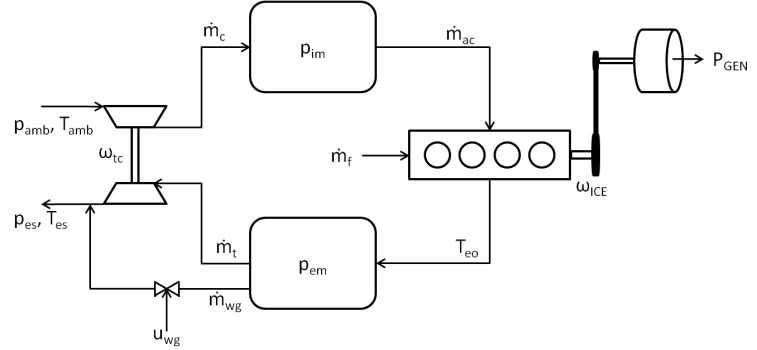
\includegraphics[width=\linewidth]{opt_diesel_model.png}
	\caption{Diagram of the diesel-electric powertrain model.}
	\label{fig:dieselmodel}
\end{figure}

In a diesel-electric powertrain the operating point of the diesel engine can be freely chosen which would potentially
decrease fuel consumption. Moreover, the electric machine has better torque characteristics. These are the main reasons
making the diesel-electric power-train concept interesting for further studies.

To investigate the fuel optimal transients of the powertrain from idling condition to a certain power level while the
accelerator pedal position is interpreted as a power level request, the following optimal control problem is solved:

\begin{equation*}
 \begin{aligned}
	\text{states}\quad x = 0, \quad \begin{pmatrix} w_{ice} \\ p_{im} \\p_{em} \\w_{tc}  \end{pmatrix}\quad = \quad \text{controls,}\quad u = \begin{pmatrix} u_{f} \\ u_{wg} \\p_{gen} \\w_{tc}  \end{pmatrix} \\
	\text{min}\;\int_{0}^{T}\dot{m}{_f} d_t
\end{aligned}
\end{equation*}

subject to

\begin{equation*}
	\begin{aligned}
		\dot{x}_1 = f_2 (x_2,x_3,u_1,u_3 ) \\
		\dot{x}_2= f_3 (x_1,x_2,x_4 ) \\
		\dot{x}_3=f_4 (x_1,x_2,x_3,u_1,u_2 ) \\
		\dot{x}_4=f_5 (x_2,x_3,x_4,u_2 ) \\
		0= f_6 (x_2,x_4 )- f_7 (x_1,x_2 ) \\
		0= f_7(x_1,x_2 ) + f_8 (x_1,u_1 )-f_9 (x_3 )-f_{10}(x_3,u_3 )  \\
		0= \frac{f_{11}(x_3)-f_{12}(x_1 )} {f_{13}(x_4 )}-f_{14} (x_4 )
\end{aligned}
\end{equation*}

\begin{equation*}
	\begin{aligned}
      54 rps \;\leq  \;  x_1  \;\leq \; 220 rps \\
      0.8 p_{amp} \;\leq \;  x_2 \; \leq \; 2P_{amb} \\
      P_{amb} \;  \leq\; x_3 \;\leq \;  3P_{amb} \\
      300rps  \; \leq \; x_4 \;\leq \;   10000 rps \\
      0 \;\leq \;u_1,u_2 \;\leq \; 1
	\end{aligned}
\end{equation*}

and boundary conditions are:

\begin{equation*}
 \begin{aligned}
	\text{at}\quad t = 0,  \begin{pmatrix} x_1 \\ x_2 \\x_3 \\x_4  \end{pmatrix} = \text{idle operating values,} \\
	\text{at}\quad t = T,  \begin{pmatrix} \dot{x}_1 \\ \dot{x}_2 \\\dot{x}_3\\\dot{x}_4 \end{pmatrix} = 0,  \begin{pmatrix} x1 \\ x2 \\x3 \\x4  \end{pmatrix} = \text{desired values} \\
	\text{and}\quad v_3 = P_{required}.
 \end{aligned}
\end{equation*}

The constraints are originated from components’ limitations and the functions $ f_i$  are described in \cite{sivertsson}.

\subsection{Model import into CasADi and NLP transcription}
\label{sec:optimizationxmlimport}

We used OpenModelica to translate Modelica/ Optimization
language extension code into an OCP in DAE and Lagrange
cost function. This OCP is then exported into an XML-based
symbolic expression format and imported into CasADi via
OpenModelica. The OCP can then be transcribed into a
nonlinear programming problem (NLP) using the approach
outlined in Section \ref{sec:totalcollocations}.

\subsection{Solution of the NLP}
\label{sec:optimizationnlp}

The NLP was solved using IPOPT \cite{wachter} running by default with the MUMPS linear solver.
The right scaling is important for a solution without oscillations.
On the other hand if the scaling does not work in all steps
then changing of the solver tolerance is helpful. The dieselmodel
is by itself well scaling in the time interval[0.32,0.5],
which is here the critical interval.

In order to cover the optimal solution of the diesel-electric
powertrain model, 140 NLP iterations for 128 sub-intervals
with the total collocation (Lobatto6 and Radau5) required by
IPOPT.

\begin{figure}
	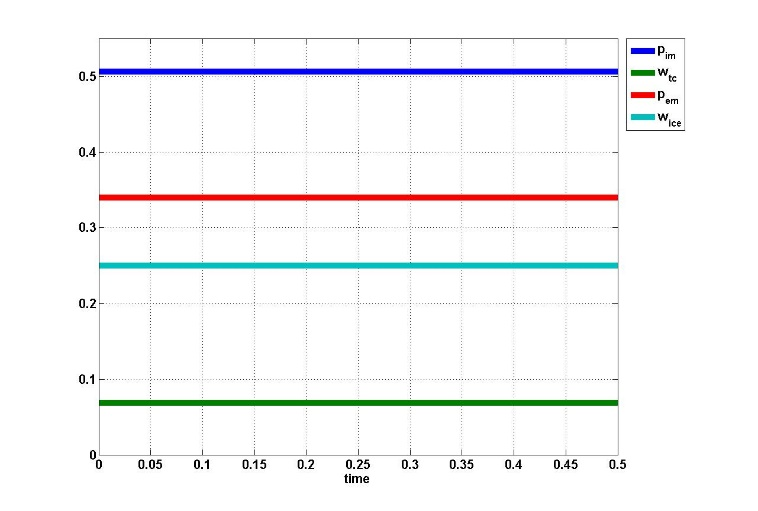
\includegraphics[width=\linewidth]{opt_initial_guess_state_variables.jpg}
	\caption{Initial guess for diesel model - state variables.}
	\label{fig:initialguessstatevariables}
\end{figure}

\begin{figure}
	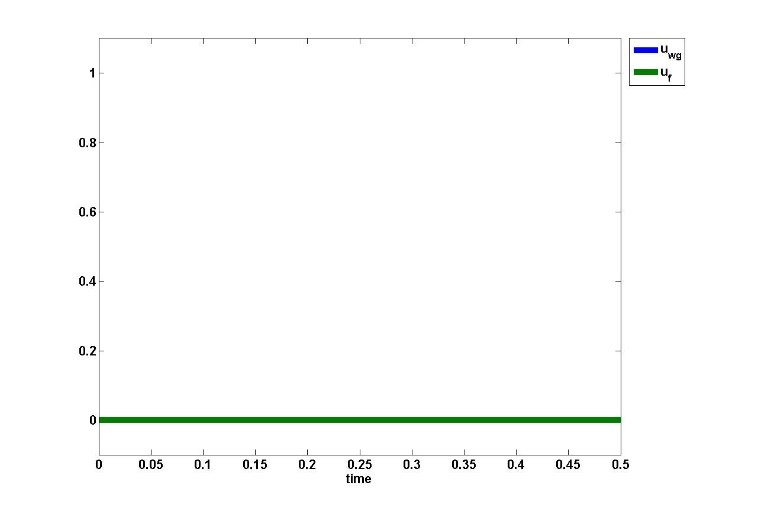
\includegraphics[width=\linewidth]{opt_initial_guess_control_variables.jpg}
	\caption{Initial guess for diesel model - control variables.}
	\label{fig:initialguesscontrolvariables}
\end{figure}


better initial guess will change the NLP iterations.
Table \ref{tab:table1} shows the total CPU time for the optimization. The calculations have been done on Dell Latitude E6410 laptop
with an Intel Core i7 processor of 2.8 GHz, 8 GB of RAM, 4M Cache, running Windows.

\begin{table}
\begin{center}
	\caption{Execution times for the diesel-electric powertrain model.} 
	\label{tab:table1} 
	\begin{tabular}{ cc } 
		\hline
		\bfseries Step & \bfseries Time  \\ 
		IPOPT (without function evaluation) & 2.140s \\ 
		NLP function evaluations & 1.158s \\ 
		\hline
	\end{tabular}
\end{center}
\end{table}

The control and state trajectories of the optimal solutions are shown in Figure \ref{fig:initialguessstatevariables} and Figure \ref{fig:initialguesscontrolvariables} respectively. The problem solved here is a minimum fuel problem for a transient 
from idle to 170 kW, for an end time of 0.5 s. For simplicity, only diesel operating condition is assumed which
means $(u_3=P_{gen} = 0)$. As it is expected, the fuel optimal results happen when engine is accelerated only near the
end of the time interval $(t\approx 0.32 s)$ to meet the end constraints while minimizing the fuel consumption.

\begin{figure}
	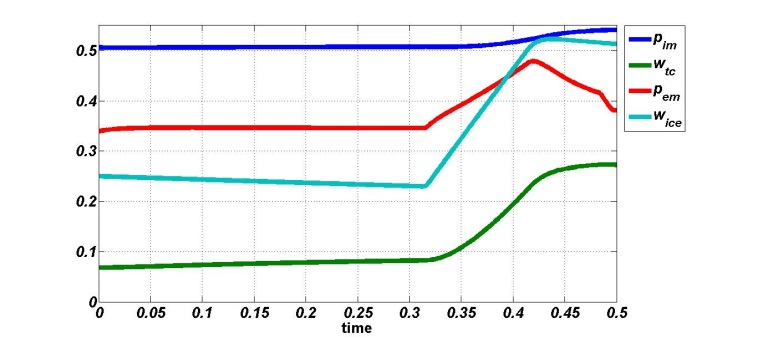
\includegraphics[width=\linewidth]{opt_result_state_variables.jpg}
	\caption{Optimization result for diesel model - state variables.}
	\label{fig:optimizationresultstatevariables}
\end{figure}

\begin{figure}
	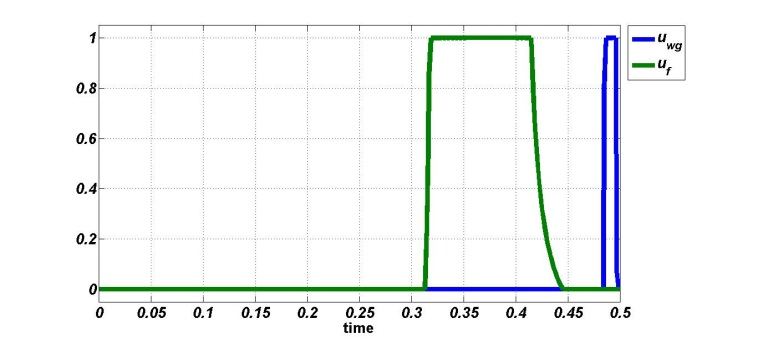
\includegraphics[width=\linewidth]{opt_result_control_variables.jpg}
	\caption{Optimization result for diesel model - control variables.}
	\label{fig:optimizationresultcontrolvariables}
\end{figure}

Amendments to the initial values, the process is robust. For this purpose, the initial values are changed slightly.

\begin{figure}
	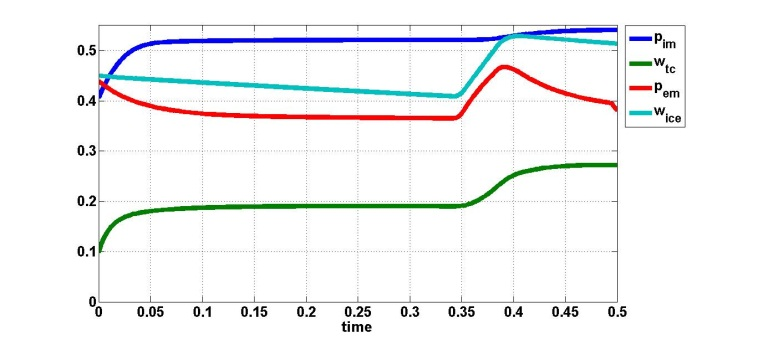
\includegraphics[width=\linewidth]{opt_result_state_variables_changed.jpg}
	\caption{Optimization result for diesel model with changed initial values - state variables.}
	\label{fig:optimizationresultchangedstatevariables}
\end{figure}

\begin{figure}
	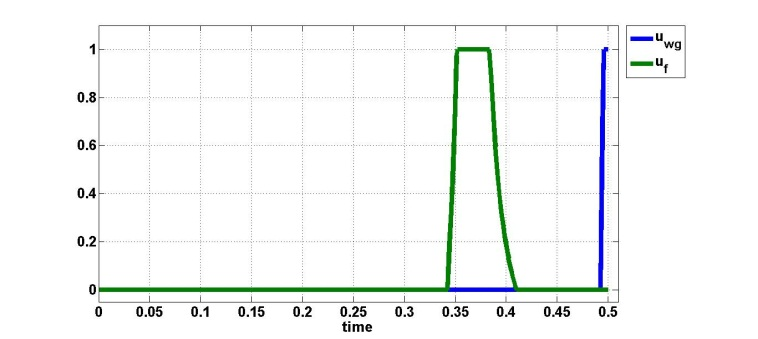
\includegraphics[width=\linewidth]{opt_result_control_variables_changed.jpg}
	\caption{Optimization result for diesel model with changed initial values - control variables.}
	\label{fig:optimizationresultchangedcontrolvariables}
\end{figure}

\subsection*{Acknowledgements}
\label{sec:optimizationacknowledgements}

This work has been partially supported by Serc, by SSF in the EDOp project and by Vinnova as well as the German
Ministry BMBF (BMBF F\"{o}rderkennzeichen: 01IS09029C) in the ITEA2 OPENPROD project and in the ITEA2 MODRIO
project. The Open Source Modelica Consortium supports the OpenModelica work.
JA and MD acknowledge support by PFV/10/002 OPTEC, GOA/10/09 and GOA/10/11, FWO G.0320.08, G.0377.09,
SBO LeCoPro; Belspo IUAP P7 DYSCO, FP7-EMBOCON (ICT-248940), SADCO (MC ITN-264735),
ERC ST HIGHWIND (259 166), Eurostars SMART, vicerp, ACCM.


%\nocite{scigen}
%We have included Paper \ref{art:scigen}

%%%%%%%%%%%%%%%%%%%%%%%%%%%%%%%%%%%%%%%%%%%%%%%%%%%%%%%%%%%%%%%%%%%%%%
%%% Intro.tex ends here


%%% Local Variables: 
%%% mode: latex
%%% TeX-master: "demothesis"
%%% End: 
